\chapter{Fundamentos Teóricos} \label{refteor}

\textcolor{red}{Este capítulo falará do referencial teórico. ele será dividido em x partes.}

\section{Detecção de bordas}

%Esta seção abordará os conceitos relacionados à detecção de bordas, assim como as técnicas de detecção utilizadas na literatura.

%\subsection{Conceitos Iniciais}
%definicao de borda

Borda é considerada a mudança abrupta ou descontinuidade em uma ou mais propriedades de sinais bidimensionais, como imagens, entre áreas vizinhas \cite{li2009markov}. Exemplos de propriedades das imagens são a intensidade, no caso de imagens em preto e branco, e os valores de R, G e B no caso de imagens coloridas.

É importante detectar estas descontinuidades pois elas podem corresponder à borda do objeto retratado, bem como mudanças na sua profundidade, iluminação ou textura \cite{descontinuidades}.

%definicao de deteccao de borda

A detecção de bordas busca, portanto, identificar onde ocorre esta descontinuidade. Sua saída é chamada mapa de bordas, uma matriz com o mesmo tamanho da imagem de origem, cujos pixeis têm valor 1 caso aquela posição, na imagem, seja correspondente a uma borda e 0 caso não seja.

Em processamento de imagens, a detecção de bordas possui as mais diversas aplicações, como por exemplo detecção de tumores no cérebro \cite{detectumor}, estudos sobre o comportamento dos pombos \cite{pigeon} e navegação espacial \cite{navegespacial}.
% LE ISSO http://citeseerx.ist.psu.edu/viewdoc/download;jsessionid=8F53C8A13258AFE7901EECFF8DFAC361?doi=10.1.1.27.1821&rep=rep1&type=pdf

\subsection{Tipos de Detectores}

%metodos de deteccao
Existem muitos métodos para detecção de bordas em imagens, mas a maioria deles pode ser dividida em dois grupos principais: os baseados no gradiente, ou primeira derivada, e os baseados no Laplaciano, ou segunda derivada \cite{tiposdetecborda}.

Os primeiros encontram as bordas baseados na localização de máximos e mínimos na primeira derivada das imagens. Entre seus exemplos mais utilizados estão o detector desenvolvido por Canny \cite{canny}, o baseado no operador de Prewitt \cite{prewitt}, o operador de Sobel \cite{citasobel} e o de Roberts \cite{roberts}.

Eles se baseiam na ideia de que uma diferença aguda no valor de uma função, no caso de imagens uma borda, gera um valor muito alto ou muito baixo em sua primeira derivada, como pode ser visto na Figura \ref{dif}. Os detectores de primeira ordem calculam o gradiente fazendo a convolução da imagem com operadores. Cada detector utiliza um operador diferente, que destaca o gradiente diferentemente.

\begin{figure}[h]
  \centering
  \subfloat[original]{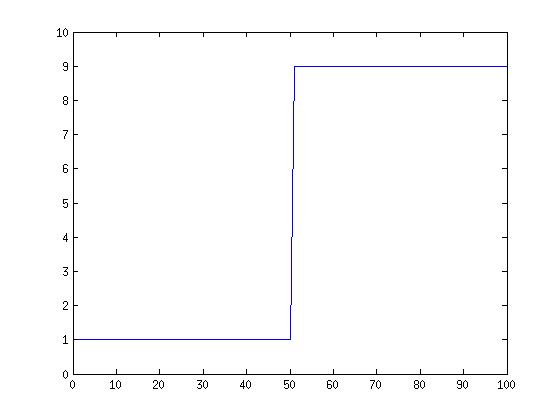
\includegraphics[width=0.45\textwidth]{figuras/fun.jpg}\label{dif:f1}}
  \hfill
  \subfloat[derivada]{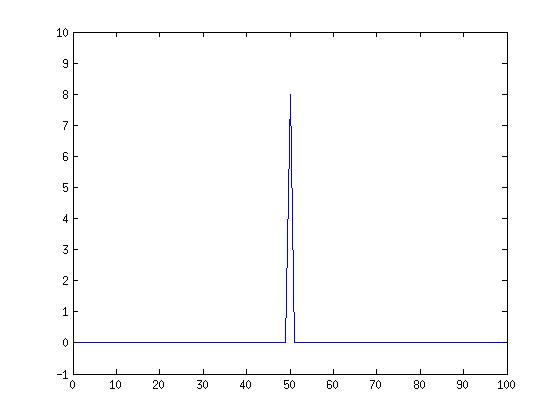
\includegraphics[width=0.45\textwidth]{figuras/fundif.jpg}\label{dif:f2}}
  \caption{uma função degrau e sua primeira derivada.}
  \label{dif}
\end{figure}

As vantagens dos métodos que utilizam a primeira derivada são a simplicidade, possibilidade de obter o ângulo do gradiente, mas têm a desvantagem de ser suscetíveis a ruído \cite{comparaborda}, portanto fazendo necessário um esquema de suavização das imagens.

\textcolor{red}{ESCREVE SOBRE OPERADORES E TÉCNICAS DE SUAVIZAÇÃO (FILTROS ETC)}
%http://citeseerx.ist.psu.edu/viewdoc/download?doi=10.1.1.301.927&rep=rep1&type=pdf

Os do segundo grupo encontram as bordas procurando onde a segunda derivada da imagem passa por zero. Dentre os detectores este grupo podemos destacar o operador de Marr-Hildreth \cite{marr} e Haralick \cite{haralick}.

A ideia deste segundo grupo de métodos é que uma borda em uma imagem gera uma passagem pelo valor zero em sua segunda derivada. Assim, os operadores utilizados neste tipo de detector visam encontrar onde a segunda derivada das imagens passa por zero.

%mais fontes
%https://www.cs.cf.ac.uk/Dave/Vision_lecture/node29.html
%http://csjournals.com/IJCSC/PDF3-2/Article_38.pdf
%http://cbcl.mit.edu/people/poggio/journals/marr-ullman-poggio-JOptSocAm-1979.pdf

\begin{figure}[h]
  \centering
  \subfloat[original]{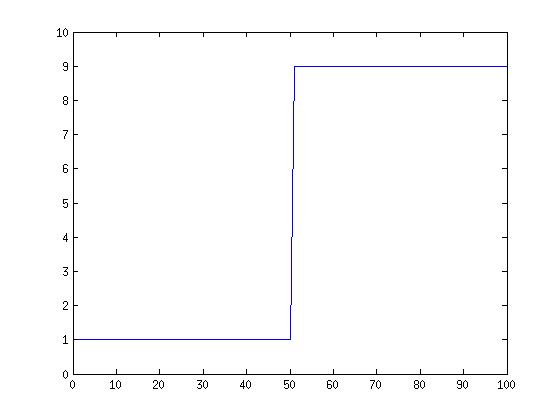
\includegraphics[width=0.45\textwidth]{figuras/fun.jpg}\label{dif:f1}}
  \hfill
  \subfloat[segunda derivada]{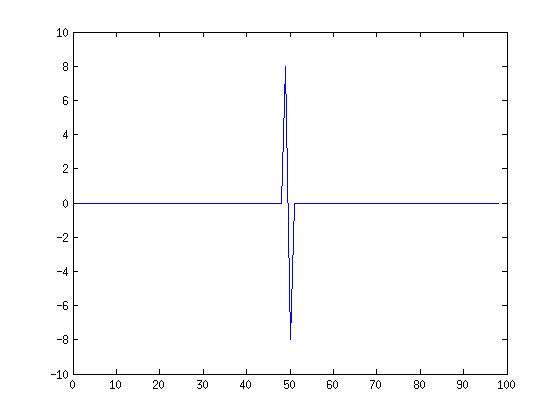
\includegraphics[width=0.45\textwidth]{figuras/fundif2.jpg}\label{dif:f2}}
  \caption{uma função degrau e sua segunda derivada.}
  \label{dif}
\end{figure}

Dentre as vantagens deste grupo de detectores está a invariância à direção da borda, mas apresenta como desvantagem uma sensibilidade a ruído ainda maior do que nos detectores de primeira ordem \cite{comparaborda}.

\section{Detecção de linhas}

% SO LE AMIG http://physics.lbl.gov/patrecog/images/A_straight_line_detection_using_principal_component_analysis.pdf
%Esta seção abordará o problema da detecção de linhas, seus conceitos principais, as principais técnicas utilizadas para este fim e um resumo sobre a transformada de Hough, base matemática para o detector utilizado nesta dissertação.

%\subsection{Conceitos Iniciais}

%baseado em: http://iie.fing.edu.uy/publicaciones/2008/GJMR08/GJMR08.pdf

Detecção de linhas é um dos problemas mais antigos e relevantes no processamento de imagens. Informação sobre segmentos de linhas em imagens é valiosa devido à maior parte dos objetos feitos por humanos ser feitos em superfícies planas e à maior parte dos objetos poderem ser simplificados em função de linhas \cite{linha00}. Em processamento de imagens, segmentos de linha são segmentos de uma linha na imagem ortogonais ao gradiente da imagem em muitos dos seus pontos \cite{linha01}. Apesar de segmentos de linha serem essencialmente bordas, esta restrição geométrica permite que sejam feitos detectores mais específicos e eficientes.

Por ser um dos problemas mais antigos da área, a detecção de linhas é base para inúmeras aplicações nas mais diversas áreas. Para citar algumas, temos compressão de imagens \cite{linhacompress}, localização de navios veleiros \cite{linhanavio}, detecção de estradas em imagens de satélites \cite{linhasestrada} e seleção de imagens relevantes \cite{linhasselecao}.

%http://citeseerx.ist.psu.edu/viewdoc/download;jsessionid=8F53C8A13258AFE7901EECFF8DFAC361?doi=10.1.1.27.1821&rep=rep1&type=pdf
%https://en.wikipedia.org/wiki/Hough_transform
%procura outras técnicas ou transformadas

%E AGORA NEGO? fala da transformada de Radon e da de Hough?

\subsection{Técnicas de Detecção}

Devido à importância da detecção de linhas, desde o início dos estudos de processamento de imagens são desenvolvidos métodos que ataquem este problema, como os baseados na transformada de Radon \cite{linhanavio,radon00} e modelos de contorno ativos \cite{contorno00,contorno01}.

Entretanto, desde que surgiu, a transformada de Hough tem se tornado um dos processos mais utilizados não só para detectar linhas, mas um dos processos mais utilizados no processamento de imagens da atualidade \cite{houghhistory}. Esta transformada, depois descoberta como um caso especial da transformada de Radon \cite{houghradon}, deu origem a inúmeras variantes que visam resolver problemas específicos com desempenho melhor que a transformada original \cite{houghalt00,houghalt01,houghalt02,houghalt03}.

A teoria geral relacionada à transformada de Hough e seu caso específico para detecção de segmentos de linha serão abordados a seguir.

\subsection{Transformada de Hough}

A transformada de Hough foi criada por P.V.C Hough para detectar padrões complexos em imagens binárias. Para atingir este objetivo, são determinados parâmetros que caracterizam estes padrões. Assim, o problema de detectar um padrão em uma imagem binária é transformado no problema de detectar um valor no espaço paramétrico \cite{houghintro01}.

%fonte: VC, H. P. (1962). U.S. Patent No. 3,069,654. Washington, DC: U.S. Patent and Trademark Office.

No caso específico de detecção de retas, a transformada de Hough funciona transformando uma linha reta em um ponto no espaço paramétrico. Os parâmetros utilizados por Hough para caracterizar uma reta no espaço $x,y$ são a inclinação $m$ e interseção $b$, portanto a reta $y = mx+b$ é representada como um ponto no espaço $m,p$.

Supondo que se tenha um conjunto de $n$ pontos em uma imagem $N = \{(x_1,y_1),(x_2,y_2),...,(x_n,y_n)\}$  e se queira descobrir a que linha eles pertencem, são computadas todas as retas que passam por aquele conjunto de pontos. Para cada reta que contém um dos pontos é computado um voto no espaço paramétrico $m,b$. Assim, a reta com maior número de votos é considerada a reta a qual os pontos pertencem. Este processo pode ser melhor representado na Figura \ref{houghpuro}

\begin{figure}[h]
  \centering
  \subfloat[imagem original]{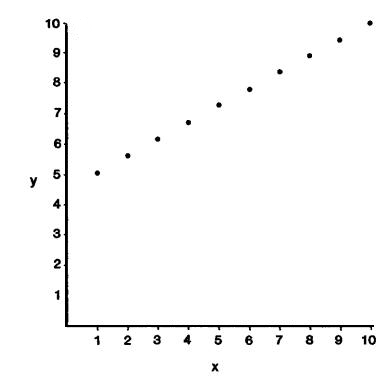
\includegraphics[width=0.4\textwidth]{figuras/houghpuro00.jpg}\label{houghpuro:f1}}
  \hfill
  \subfloat[representação no espaço paramétrico]{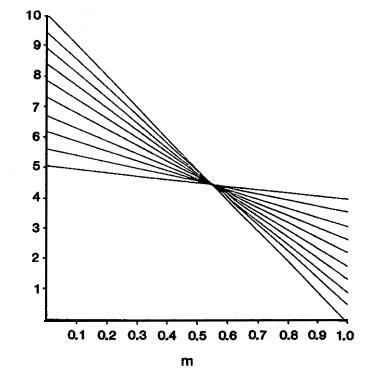
\includegraphics[width=0.4\textwidth]{figuras/houghpuro01.jpg}\label{houghpuro:f2}}
  \caption{imagem com pontos colineares e sua representação no espaço $m,b$. Adaptado de \cite{houghintro01}.}
  \label{houghpuro}
\end{figure}

Entretanto, a parametrização no espaço $m,b$ não consegue representar corretamente linhas verticais ou próximas desta inclinação, como perceberam Duda e Hart em seu influente artigo \cite{houghintro02}. A fim de eliminar estes problemas, eles propuseram uma nova parametrização para a transformada de Hough. Nela, as retas no espaço $x,y$ são representadas no espaço $\rho,\theta$, onde $\rho$ é a distância entre a origem da imagem e a reta, pelo seu ponto mais próximo, e $\theta$ é o ângulo que a normal à reta faz com o eixo $x$. A equação da reta, portanto, é dada por: 

$$\rho = x cos \theta +y sin \theta $$ 

%fonte: Duda, R. O., & Hart, P. E. (1972). Use of the Hough transformation to detect lines and curves in pictures. Communications of the ACM, 15(1), 11-15.

%FIGURA COM UMA RETA MOSTRANDO RHO E THETA

\begin{figure} [h]
\centering
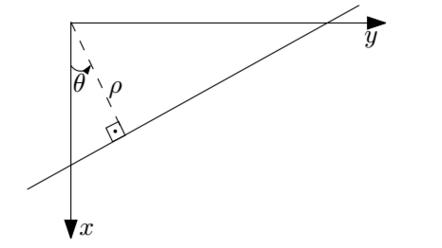
\includegraphics[width = 0.6\textwidth]{figuras/hough.jpg} \label{hough} \caption{Representação paramétrica de Hough. Adaptado de \cite{hough00}}
\end{figure} 

%imagem de: Jung, C. R., & Schramm, R. (2004, October). Rectangle detection based on a windowed Hough transform. In Computer Graphics and Image Processing, 2004. Proceedings. 17th Brazilian Symposium on (pp. 113-120). IEEE.

Assim, dado um pixel de borda, para cada possível reta que passe por ele, é computado um ponto no espaço $(\rho,\theta)$. O conjunto de linhas possíveis passando por um determinado ponto forma um sinusoide naquele espaço. Com dois ou mais pontos na imagem pertencendo à mesma linha, as sinusoides que os representam se tocam justamente no ponto que representa a mesma. Isto é melhor representado na imagem \ref{houghlinhas}, que mostra uma imagem com dois pontos brancos e sua representação no espaço de Hough.

%FIGURA REPRESENTANDO DOIS PONTOS LIGADOS À MESMA LINHA E O SEU ESPAÇO PARAMÉTRICO

\begin{figure}[h]
  \centering
  \subfloat[imagem original]{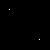
\includegraphics[width=0.35\textwidth]{figuras/houghpts0000.jpg}\label{houghlinhas:f1}}
  \hfill
  \subfloat[representação no espaço de Hough]{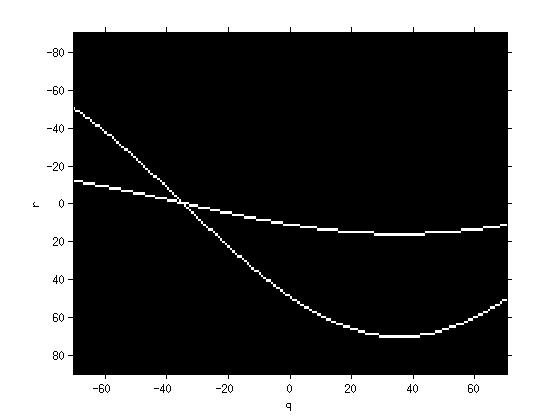
\includegraphics[width=0.5\textwidth]{figuras/houghpts0001.jpg}\label{houghlinhas:f2}}
  \caption{imagem com dois pontos e a representação paramétrica.}
  \label{houghlinhas}
\end{figure}

\section{Detecção de Retângulos}

%\subsection{Conceitos Iniciais}

%http://www.cse.cuhk.edu.hk/~khwong/c15_Multiple_quadrilateral_detection_iciea15.pdf
%http://cbcl.mit.edu/people/poggio/journals/mohan-poggio-IEEE-PAMI-2001.pdf
%http://mame.myds.me/bitsavers/pdf/dec/tech_reports/CRL-2001-1.pdf

%conceito de retangulo
Um objeto retangular pode ser considerado um caso especial de objeto quadrangular, que é definido \cite{objquadrangular01} como um objeto delimitado por quatro segmentos de reta distintos pertencentes à mesma imagem, lifados por quatro vértices. O retângulo é um caso especial em que os lados conectados são perpendiculares.

%reconhecimento de retangulos
A detecção de retângulos é um problema antigo do processamento de imagens e reconhecimento de padrões. É um problema relevante devido ao fato de muitos dos objetos feitos por mãos humanas terem bordas retangulares \cite{mrf}. 

%importância aplicacoes
Assim como a detecção de bordas e de segmentos de linha, este também é um problema que, de tão geral, tem aplicações em campos diversos, tais como detecção de prédios em imagens de satélite \cite{prediosatelite,prediosatelite00}, detecção de placas de trânsito em tempo real \cite{placatransito} e detecção de partículas em imagens microscópicas \cite{detecparticulas}. %Building Detection in a Single Remotely Sensed Image with a Point Process of Rectangles

\subsection{Técnicas de Detecção}

%http://www.cs.utexas.edu/~bajaj/papers/2004/journal/sdarticle02.pdf
%https://hal.archives-ouvertes.fr/hal-00422588/document
%http://www.cse.cuhk.edu.hk/~khwong/c15_Multiple_quadrilateral_detection_iciea15.pdf
%http://cbcl.mit.edu/people/poggio/journals/mohan-poggio-IEEE-PAMI-2001.pdf
%http://mame.myds.me/bitsavers/pdf/dec/tech_reports/CRL-2001-1.pdf
%https://hal.inria.fr/file/index/docid/481019/filename/benedekICPR10.pdf
%http://koasas.kaist.ac.kr/bitstream/10203/23905/1/OMNIVIS_cameraready_001.pdf
%http://en.cnki.com.cn/Article_en/CJFDTOTAL-JSJC201208054.htm
%http://ieeexplore.ieee.org/xpl/login.jsp?tp=&arnumber=5876761&url=http%3A%2F%2Fieeexplore.ieee.org%2Fxpls%2Fabs_all.jsp%3Farnumber%3D5876761
%http://www.csd.uwo.ca/faculty/olga/Courses/Fall2012/CS9840/PossibleStudentPapers/RoadSigns2004.pdf
%http://ieeexplore.ieee.org/search/searchresult.jsp?queryText=sign%20image%20quadrilateral%20object&newsearch=true
%http://imaging.utk.edu/publications/papers/1995/abidi_pami95.pdf
%https://www.google.com.br/search?q=quadrangular+detection+based+on+a+robust+line+tracker+using&oq=quadrangular+detection+based+on+a+robust+line+tracker+using&gs_l=serp.3...4642.14775.0.15376.19.17.0.0.0.0.481.2210.2-4j1j2.7.0....0...1c.1.64.serp..12.2.726.kDzNb5CnicE

A maioria das técnicas para detecção de retângulos é baseada na transformada de Hough \cite{houghintro00}. Foi descoberto que esta transformada pode ser utilizada para detectar formas arbitrárias, apesar de ser mais famosa pela detecção de linhas \cite{houghgeral}. Assim, surgiram inúmeras variações da transformada visando resolver exclusivamente este problema, tal como a Transformada Retangular de Hough (RHT) \cite{houghrectangle} e transformada com janelas \cite{hough00}.

Outras técnicas envolvem análise de informações básicas de linhas. Um exemplo é encontrado em \cite{primitivas}, onde segmentos de linha são encontrados e agrupados de forma que a técnica consiga descobrir se fazem parte ou não de objetos retangulares. Outro é visto em \cite{primitivas00}, onde as informações espaciais das linhas detectadas são utilizadas para encontrar linhas paralelas entre si e, posteriormente, retângulos.

Um grupo de técnicas promissoras é baseado na ideia de que pode-se encarar o problema de detecção de retângulos como um problema de otimização \cite{rectgenetic00}, o que gerou uma série de implementações da detecção de retângulos baseada em algoritmos genéticos 
\cite{rectgenetic01,rectgenetic02}.

\begin{comment}

cara, o lance é que eu não sei se esta seção precisa entrar. eu acho importante falar da inspeção de monitores, mas não sei se vai ser nesse capítulo, já que trato dela no cap 5

\section{Inspeção Automática de Monitores}

%http://ieeexplore.ieee.org/stamp/stamp.jsp?arnumber=5439135
%http://ieeexplore.ieee.org/stamp/stamp.jsp?arnumber=4960847
%http://ieeexplore.ieee.org/stamp/stamp.jsp?tp=&arnumber=4767309&tag=1
%http://ieeexplore.ieee.org/stamp/stamp.jsp?tp=&arnumber=254542

\subsection{Conceitos Iniciais}

%conceito de tela??

%inspeção de monitores, como é feita etc

%aplicações????????
\subsection{Técnicas de Inspeção}

\end{comment}